\chapter{Results and Analysis}
\label{ch:5}
The sections run in the order of the argument, not the order the runs were made: the in-sample audit
(5.1 to 5.5), its mechanism (5.6), the out-of-sample result and its curve (5.7 and 5.8), what never
transferred (5.9), what survives for practice (5.10), and the decision each research question comes
to on this evidence (5.11). Every difference is a paired bootstrap interval; single-seed rows are
marked and treated as indicative.
\section{The Teachers Clear the Bar}
\label{sec:5.1}
\begin{table}[htbp]
\centering
\small
\caption[Teachers after task adaptation]{Teachers after task adaptation, with the classical floor. The training loss is the last epoch's cross-entropy on the split the students are distilled on; the probe columns are the share of each probe the model assigns to any abusive class, which is its argmax decision rather than a threshold on $p(\text{abusive})$.}
\label{tab:teachers}
\begin{adjustbox}{max width=\textwidth}
\begin{tabular}{lcccccc}
\toprule
Teacher & Macro-F1 & Accuracy & ECE & Training loss, last epoch & Benign-sarcasm FPR & Ironic-abuse recall \\
\midrule
BERT-large & 0.8973 & 0.9075 & 0.056 & 0.033 & 0.224 & 0.585 \\
Implicit specialist, task-adapted & 0.8931 & 0.9043 & 0.072 & 0.061 & 0.263 & 0.678 \\
RoBERTa-irony, task-adapted & 0.8926 & 0.9050 & 0.067 & 0.077 & 0.294 & 0.718 \\
HateBERT, task-adapted & 0.8887 & 0.9011 & 0.076 & 0.059 & 0.317 & 0.696 \\
DeBERTa-v3-base & 0.8720 & 0.8867 & 0.053 & 0.227 & 0.409 & 0.773 \\
TF-IDF + logistic regression & 0.8798 & 0.8930 & -- & -- & -- & -- \\
\bottomrule
\end{tabular}
\end{adjustbox}
\end{table}

Table~\ref{tab:teachers} reports the teachers after task adaptation. Three of the original four beat
the fine-tune-only headline student and the classical floor, so the pre-registered stop rule passes.
DeBERTa-v3-base sits below the floor and is retained only as the heterogeneous committee member,
which is what it is there to test. The implicit specialist, trained on different data under a
different label scheme, lands within 0.005 of the other three after adaptation. Two columns of this
table carry the rest of the paper. The training losses say that every task-adapted teacher has, by
its last epoch, assigned the gold label a probability near one on the split the student will be
distilled on (Section~\ref{sec:5.6}). And the probe columns already show the pattern
Section~\ref{sec:5.9} makes precise: ordered by false-positive rate on harmless sarcasm, the
teachers are almost exactly ordered by recall on ironic abuse.
\section{In Sample, Distillation Raises Every Student by Less Than the Test Set Can Resolve}
\label{sec:5.2}
Table~\ref{tab:main} gives the in-sample grid: test macro-F1 of every student under every objective
and committee, against a classical floor of 0.8798.

\begin{table}[htbp]
\centering
\small
\caption[In-sample distillation on the five students]{In-sample distillation: test macro-F1 of the five students under each objective and committee, mean over three seeds. The classical floor is 0.8798. Standard deviations over seeds run from 0.0002 to 0.0078 and are in the generated table \texttt{paper/tables/main.csv}; the paired intervals are in Appendix~\ref{app:significance}.}
\label{tab:main}
\begin{adjustbox}{max width=\textwidth}
\begin{tabular}{lccccccc}
\toprule
Student & Params & Fine-tune only & Single-teacher & Uniform & D-MTHD & Uniform + DeBERTa & D-MTHD + DeBERTa \\
\midrule
BERT-mini & 11.2M & 0.8393 & 0.8405 & 0.8385 & 0.8378 & 0.8378 & 0.8373 \\
BERT-small & 28.8M & 0.8469 & 0.8488 & 0.8505 & 0.8471 & 0.8509 & 0.8477 \\
DistilBERT & 67.0M & 0.8907 & 0.8963 & 0.8960 & 0.8960 & 0.8975 & 0.8966 \\
DeBERTa-v3-xsmall & 70.8M & 0.8825 & 0.8865 & 0.8862 & 0.8833 & 0.8847 & 0.8828 \\
BiLSTM & 10.4M & 0.8693 & 0.8748 & 0.8761 & 0.8732 & 0.8760 & 0.8764 \\
\bottomrule
\end{tabular}
\end{adjustbox}
\end{table}

Best distilled configuration against fine-tune-only: BERT-mini +0.0012 [$-$0.0057, +0.0079],
BERT-small +0.0040 [$-$0.0058, +0.0126], DistilBERT +0.0068 [$-$0.0013, +0.0139], DeBERTa-v3-xsmall
+0.0040 [$-$0.0024, +0.0109], BiLSTM +0.0071 [$-$0.0039, +0.0195]. Five of five positive, which is
the result the control was added to test; and none of the five intervals excludes zero, nor does any
of the 27 in-sample distillation-against-fine-tuning comparisons in the grid. Taking the best of six
configurations per student also flatters the difference. The supportable claim is the modest one: in
sample, distillation moves every student in the same direction, by 0.001 to 0.007 macro-F1, which a
test set of 4,326 posts cannot resolve.

Two students deserve a remark. The most heterogeneous student, the BiLSTM, gains the most, and the
student that shares the teachers' architecture most closely, BERT-mini, gains the least; the
hidden-state term, the only part of the objective that architectural similarity could help, is worth
+0.0009 on BERT-mini. Nothing in this grid supports a preference for homogeneous student and
teachers. And on BERT-mini no distilled configuration beats the no-teacher control by more than the
seeds' own spread: candidate minus fine-tune-only is $-$0.0015 [$-$0.0076, +0.0048] for D-MTHD,
$-$0.0007 [$-$0.0074, +0.0058] for uniform, +0.0012 [$-$0.0057, +0.0079] for single-teacher,
$-$0.0019 [$-$0.0082, +0.0041] with the DeBERTa committee, $-$0.0003 [$-$0.0080, +0.0075] and
$-$0.0019 [$-$0.0093, +0.0049] with the specialist committee under averaging and weighting.

The efficiency claim sits in this table. DistilBERT with a uniform heterogeneous committee reaches
0.8975 against BERT-large's 0.8973 at a fifth of the parameters and latency
(Section~\ref{sec:5.10}). We state that as parity, not as the student beating the teacher.
\section{Per-Instance Weighting Does Not Differ from Uniform Averaging at Any Temperature}
\label{sec:5.3}
\begin{table}[htbp]
\centering
\small
\caption[Per-instance weighting minus uniform averaging]{Per-instance weighting minus uniform averaging, with and without the DeBERTa teacher; paired bootstrap 95\% intervals.}
\label{tab:dmthd-uniform}
\begin{adjustbox}{max width=\textwidth}
\begin{tabular}{lcc}
\toprule
Student & D-MTHD minus uniform & Same, with DeBERTa \\
\midrule
BERT-mini & $-$0.0007 [$-$0.0074, +0.0061] & $-$0.0005 [$-$0.0067, +0.0054] \\
BERT-small & $-$0.0034 [$-$0.0106, +0.0036] & $-$0.0032 [$-$0.0100, +0.0033] \\
DistilBERT & +0.0000 [$-$0.0079, +0.0082] & $-$0.0010 [$-$0.0087, +0.0069] \\
DeBERTa-v3-xsmall & $-$0.0029 [$-$0.0086, +0.0029] & $-$0.0019 [$-$0.0108, +0.0108] \\
BiLSTM & $-$0.0029 [$-$0.0116, +0.0056] & +0.0004 [$-$0.0072, +0.0081] \\
\bottomrule
\end{tabular}
\end{adjustbox}
\end{table}

Table~\ref{tab:dmthd-uniform} sets the weighting against averaging on every student. Without the
DeBERTa teacher four differences are negative and one is a tie; with it, four are negative and one
positive. Every interval contains zero. On the headline student the ablation that removes the
weighting altogether scores 0.8386 against 0.8385 for full D-MTHD on the same seed.

The obvious objection is that at $\tau = 1$ the weights are nearly uniform, 0.332 / 0.337 / 0.331
against 0.333, so the two objectives coincide by arithmetic. The sweep therefore reaches $\tau =
0.05$ (Table~\ref{tab:tau}, Figure~\ref{fig:tau}).

\begin{table}[htbp]
\centering
\small
\caption[Teacher weights and score across the temperature sweep]{The weighting-temperature sweep on BERT-mini: mean weight of each teacher over the training split, and test macro-F1 of the first seed.}
\label{tab:tau}
\begin{adjustbox}{max width=\textwidth}
\begin{tabular}{lcc}
\toprule
$\tau$ & Mean weights, BERT-large / HateBERT / irony & Test macro-F1, seed 1 \\
\midrule
0.05 & 0.318 / 0.356 / 0.326 & 0.8392 \\
0.1 & 0.323 / 0.349 / 0.328 & 0.8388 \\
0.2 & 0.327 / 0.344 / 0.329 & 0.8385 \\
0.5 & 0.330 / 0.340 / 0.330 & 0.8390 \\
1 (default) & 0.332 / 0.337 / 0.331 & 0.8385 \\
2 & 0.332 / 0.336 / 0.332 & 0.8390 \\
5 & 0.333 / 0.334 / 0.333 & 0.8389 \\
Uniform averaging & 0.333 each & 0.8372 \\
Fine-tune only & -- & 0.8394 \\
\bottomrule
\end{tabular}
\end{adjustbox}
\end{table}

\begin{figure}[htbp]
\centering
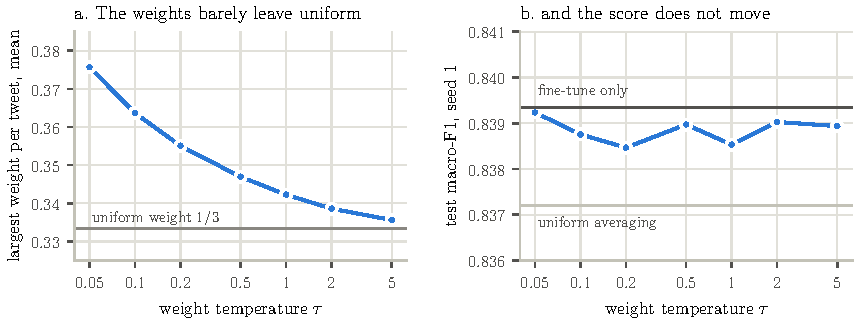
\includegraphics[width=\textwidth]{figures/fig_tau.pdf}
\caption[The weighting-temperature sweep on BERT-mini]{The weighting-temperature sweep on BERT-mini. (a) Even at $\tau = 0.05$ the largest teacher weight on a tweet averages 0.376 against a uniform 0.333. (b) Test macro-F1 of the first seed stays within 0.0007 across a hundredfold range of $\tau$, below fine-tuning at every value.}
\label{fig:tau}
\end{figure}

Across a hundredfold range of temperature the score stays inside 0.0007 and below fine-tune-only at
every value; the sharpest setting differs from the default by +0.0007 [$-$0.0008, +0.0023] and from
uniform averaging by +0.0020 [$-$0.0042, +0.0077]. The weights barely sharpen: even at $\tau = 0.05$
the heaviest teacher averages 0.356.

\textbf{Ablations and sweeps say the same.} BERT-mini, one seed, against full D-MTHD at 0.8378:
randomly initialised student 0.7905 ($-$0.0473); no auxiliary irony head 0.8364 ($-$0.0014); no
hidden-state term 0.8369 ($-$0.0009); uniform weights 0.8386 (+0.0008); per-batch weights 0.8389
(+0.0011); the specialist alone 0.8392 (+0.0014); pre-trained on the implicit corpus 0.8377
($-$0.0001). Removing components of the method costs at most 0.0014 and in three cases improves the
score; removing pre-training costs 0.047, and against fine-tune-only on the same seed it is the one
in-sample difference in the grid whose interval excludes zero, $-$0.0488 [$-$0.0603, $-$0.0376].
Hyper-parameters behave the same way, against 0.8385 at the defaults on the same seed: $T \in \{1,
2, 8\}$ gives 0.8386 / 0.8402 / 0.8391, $\alpha \in \{0.2, 0.6\}$ 0.8386 / 0.8394, $\delta \in
\{0.1, 0.5\}$ 0.8389 / 0.8399. The objective is flat in every direction we can move it, and adding a
DeBERTa-v3 teacher to the homogeneous committee changes the five students by $-$0.0005, +0.0006,
+0.0032, $-$0.0005 and +0.0006.
\section{The Committee Is Worth More Than Its Best Member, and the Student Receives None of It}
\label{sec:5.4}
Table~\ref{tab:committee} scores the teachers' saved test probabilities directly, before any student
is involved.

\begin{table}[htbp]
\centering
\small
\caption[Combining the teachers directly on the test set]{Combining the teachers directly on the test set, before any student is trained: macro-F1 of each combination rule and the oracle's accuracy.}
\label{tab:committee}
\begin{adjustbox}{max width=\textwidth}
\begin{tabular}{lccccccc}
\toprule
Committee & Best single & Uniform mean & Confidence-weighted & Entropy-weighted & Most confident teacher & Stacked gate (5-fold CV) & Oracle accuracy \\
\midrule
Homogeneous (3) & 0.8973 & 0.9026 & 0.9018 & 0.9023 & 0.9015 & 0.9046 & 0.9454 \\
+ implicit specialist (4) & 0.8973 & 0.9000 & 0.9005 & 0.9011 & 0.9011 & 0.9043 & 0.9494 \\
+ DeBERTa (4) & 0.8973 & 0.9051 & 0.9055 & 0.9052 & 0.9005 & 0.9055 & 0.9526 \\
All five & 0.8973 & 0.9036 & 0.9046 & 0.9030 & 0.9000 & 0.9041 & 0.9552 \\
\bottomrule
\end{tabular}
\end{adjustbox}
\end{table}

Uniform averaging of the committee beats the best teacher by 0.3 to 0.8 macro-F1. No combination
that needs no gold label at inference improves on the uniform mean by more than 0.005, and neither
does a stacked logistic-regression gate fitted to the concatenated teacher probabilities by
five-fold cross-validation over the test set, which is as favourable a test of learned routing as
can be made without touching the training data. The oracle that picks a correct teacher whenever one
exists sits at 0.945 to 0.955 accuracy, against 0.9075 for BERT-large. That headroom is real and it
is unreachable from the teachers' outputs: where the teachers disagree, 10 to 14 per cent of the
test set, some teacher is right on about 90 per cent of items and the uniform mean on 55 to 62, and
their probabilities do not say which. A corrected reliability signal therefore has a ceiling of
under half a point of macro-F1 over uniform averaging on this committee, in or out of sample.

The teachers are not diverse enough for a weighting to have work to do, and adaptation is what made
them so (Table~\ref{tab:agreement}, Figure~\ref{fig:agreement}).

\begin{table}[htbp]
\centering
\small
\caption{Agreement between the task-adapted teachers on the test set.}
\label{tab:agreement}
\begin{adjustbox}{max width=\textwidth}
\begin{tabular}{lccc}
\toprule
Teacher pair & Cohen's kappa & Disagreement & Error overlap \\
\midrule
BERT-large, HateBERT & 0.920 & 6.7\% & 0.710 \\
BERT-large, irony & 0.922 & 6.4\% & 0.712 \\
BERT-large, DeBERTa-v3 & 0.893 & 8.9\% & 0.712 \\
HateBERT, irony & 0.916 & 7.0\% & 0.673 \\
HateBERT, DeBERTa-v3 & 0.889 & 9.2\% & 0.673 \\
irony, DeBERTa-v3 & 0.900 & 8.3\% & 0.730 \\
BERT-large, implicit specialist & 0.924 & 6.4\% & 0.710 \\
\textbf{HateBERT, implicit specialist} & \textbf{0.962} & \textbf{3.1\%} & \textbf{0.843} \\
irony, implicit specialist & 0.918 & 6.8\% & 0.689 \\
implicit specialist, DeBERTa-v3 & 0.889 & 9.2\% & 0.691 \\
\bottomrule
\end{tabular}
\end{adjustbox}
\end{table}

\begin{figure}[htbp]
\centering
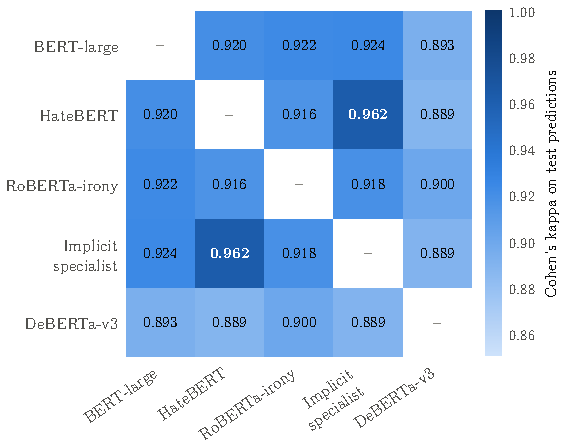
\includegraphics[width=\textwidth]{figures/fig_agreement.pdf}
\caption[Pairwise agreement between the task-adapted teachers]{Cohen's kappa between the task-adapted teachers' test predictions. Every pair agrees above 0.88, and the implicit specialist agrees with HateBERT, the checkpoint it was trained from, at 0.962. A per-instance weighting has to work inside what is left.}
\label{fig:agreement}
\end{figure}

The original four teachers are all right on 83.2 per cent of the test set and all wrong on the same
4.7 per cent. A per-instance weighting can only express a preference where its members disagree, at
most one instance in seven here, and on about half of the best teacher's errors no member is right
to prefer. The committee was chosen for complementary expertise, and after task adaptation on the
same corpus its members converged to near-identical behaviour. Task adaptation is what makes a
sarcasm model's logits comparable with an abuse model's, and it is also what removes the diversity
the combination was meant to exploit. \textbf{Task adaptation buys comparability and spends
diversity}, and any cross-task committee faces the trade.

The students do not receive even the 0.3 to 0.8 that the committee has. Uniform multi-teacher
against single-teacher distillation is $-$0.0019 [$-$0.0077, +0.0038], +0.0017 [$-$0.0070, +0.0115],
$-$0.0003 [$-$0.0070, +0.0060], $-$0.0003 [$-$0.0072, +0.0070] and +0.0014 [$-$0.0073, +0.0099]
across the five students. A better label on the same 34,607 training texts does not make a better
student, and Section~\ref{sec:5.6} says why: on those texts the label is not better.
\section{A Teacher That Has Seen Implication Labelled Does Not Help Either}
\label{sec:5.5}
The implicit specialist is the sharpest case of the previous section. It learned from a different
corpus under a different label scheme, and it comes back from adaptation as the closest thing in the
committee to HateBERT, the model it started from: kappa 0.962, disagreement on 3.1 per cent of the
test set, 84 per cent of HateBERT's errors made by the specialist as well. It raises the oracle over
the committee only from 0.9526 to 0.9552. Table~\ref{tab:specialist} gives the specialist and its
two controls on the headline student.

\begin{table}[htbp]
\centering
\small
\caption{The implicit specialist and its controls on BERT-mini.}
\label{tab:specialist}
\begin{adjustbox}{max width=\textwidth}
\begin{tabular}{lcccc}
\toprule
Configuration & Seeds & Macro-F1 & F1 on other\_cyberbullying & Sarcasm-discrimination AUC (seed 1) \\
\midrule
Fine-tune only & 3 & 0.8393 $\pm$ 0.0003 & 0.707 & 0.773 \\
Uniform, homogeneous committee & 3 & 0.8385 $\pm$ 0.0018 & 0.700 & 0.774 \\
Uniform, + implicit specialist & 3 & 0.8390 $\pm$ 0.0035 & 0.699 & 0.768 \\
D-MTHD, homogeneous committee & 3 & 0.8378 $\pm$ 0.0011 & 0.705 & 0.773 \\
D-MTHD, + implicit specialist & 3 & 0.8373 $\pm$ 0.0025 & 0.697 & 0.768 \\
Specialist alone, no committee & 1 & 0.8392 & 0.709 & 0.767 \\
Pre-trained on the implicit corpus, no teacher & 1 & 0.8377 & 0.705 & 0.756 \\
\bottomrule
\end{tabular}
\end{adjustbox}
\end{table}

Adding the specialist changes macro-F1 by +0.0005 [$-$0.0059, +0.0064] under averaging and $-$0.0005
[$-$0.0069, +0.0055] under weighting; F1 on the class that holds indirect abuse and the
discrimination AUC both fall slightly. Neither control does better: the specialist alone sits within
0.0002 of the no-teacher student, and putting the implicit corpus into the student directly, by
pre-training on it, gives the lowest discrimination AUC of the in-sample models analysed.

The weights do lean towards the specialist, a little, and less than towards HateBERT. Measured in
the committee the students trained with, on the training split, as mean weight on
other\_cyberbullying minus mean weight on the four targeted classes, against a uniform weight of
0.25 (Table~\ref{tab:routing}).

\begin{table}[htbp]
\centering
\small
\caption[Routing contrast in the committee with the specialist]{Routing contrast in the committee with the specialist: mean weight on other\_cyberbullying minus mean weight on the four targeted classes, with 95\% bootstrap intervals. The uniform weight is 0.25.}
\label{tab:routing}
\begin{adjustbox}{max width=\textwidth}
\begin{tabular}{lcc}
\toprule
Teacher (committee with the specialist) & $\tau$ = 0.05 & $\tau$ = 1 \\
\midrule
HateBERT & +0.0235 [+0.0209, +0.0260] & +0.0044 [+0.0034, +0.0055] \\
Implicit specialist & +0.0187 [+0.0163, +0.0212] & +0.0027 [+0.0018, +0.0036] \\
RoBERTa-irony & $-$0.0075 [$-$0.0101, $-$0.0048] & $-$0.0011 [$-$0.0021, +0.0001] \\
BERT-large & $-$0.0347 [$-$0.0375, $-$0.0317] & $-$0.0060 [$-$0.0074, $-$0.0046] \\
\bottomrule
\end{tabular}
\end{adjustbox}
\end{table}

With tens of thousands of instances almost any contrast excludes zero, so the size is the evidence.
At the temperature the students trained with, the specialist's shift is a hundredth of the uniform
weight, and it is not specific to the specialist: HateBERT, which never saw the implicit corpus,
gains more, as the kappa predicts. And because the weights come from cross-entropy against the gold
label, a shift says only that a teacher fits other\_cyberbullying better than the targeted classes,
not that it reads implication. On this corpus, a teacher that has learned implication from labelled
data passes nothing a compact student's decisions can use, whether weighted, averaged, used alone or
replaced by pre-training on its data.
\section{Why Nothing Moved: The Soft Labels Are the Gold Labels in Sample}
\label{sec:5.6}
The weights are computed from cached teacher logits on the training split, the split each teacher
was fine-tuned on, and the student is distilled on the same split. By their last epoch the teachers'
training losses are 0.033 (BERT-large), 0.059 (HateBERT), 0.077 (irony), 0.061 (implicit specialist)
and 0.227 (DeBERTa-v3-base). On the data the weights are read from, every task-adapted teacher
assigns the gold label a probability near one on nearly every instance, cross-entropy differences
between them are a few hundredths, and the softmax of Section~\ref{sec:3.2} is flat at any
temperature that does not amplify noise. The one teacher that did not memorise the split, DeBERTa,
is the one whose weight moves (0.233 in a committee of four). The reliability signal is measuring
memorisation, not reliability, and this is a property of the error-weighted family \cite{wu2021one,
zhang2022confidence}, not of our implementation: any scheme that scores reliability against the gold
label on the training data will find every fine-tuned teacher equally reliable there.

The same fact bears on the distillation itself. On the training split the teachers' soft labels are
close to the one-hot gold labels, so the KL term carries little that the cross-entropy term does
not, and single-teacher, uniform and weighted distillation all reduce to fine-tuning with a slightly
smoothed target. This is the hazard of distilling a memorising teacher on its own training data
\cite{stanton2021does, beyer2022knowledge}, and it explains Section~\ref{sec:5.4} from the student's
side: the committee's half point exists on the test set, where the teachers are uncertain, and not
on the training set, where they are not. It also says where to look. If a teacher's soft labels
carry information only where the teacher is uncertain, the student should be distilled on text the
teacher has never fitted. The rest of the results test that sentence.
\section{Out of Sample, the Gain Appears, and It Is in the Data, Not the Committee}
\label{sec:5.7}
A transfer set of 42,013 unlabelled tweets (Section~\ref{sec:4.4}) was appended to training; on
those rows the student has no gold label and trains on the committee's soft labels and hidden states
alone. Table~\ref{tab:oos} reports five arms on BERT-mini, three seeds each, beside the in-sample
runs of the same objectives; the predictions were written before the run and are scored in
Appendix~\ref{app:predictions}.

\begin{table}[htbp]
\centering
\small
\caption[Out-of-sample distillation on BERT-mini]{Out-of-sample distillation on BERT-mini with the 42,013-tweet transfer set: the same objectives with and without the unlabelled rows, three seeds each. The labelled-split column gives each objective's in-sample twin; for the out-of-sample-weighted arm that twin is D-MTHD, because the weighting differs only where there are no labels.}
\label{tab:oos}
\begin{adjustbox}{max width=\textwidth}
\begin{tabular}{lccc}
\toprule
Objective & Labelled split only & + transfer set & Gain over fine-tune only \\
\midrule
Fine-tune only & 0.8393 $\pm$ 0.0003 & -- & -- \\
Single teacher (BERT-large) & 0.8405 $\pm$ 0.0017 & 0.8466 $\pm$ 0.0016 & +0.0073 [$-$0.0003, +0.0150] \\
Uniform committee & 0.8385 $\pm$ 0.0018 & 0.8462 $\pm$ 0.0016 & +0.0070 [$-$0.0001, +0.0144] \\
Uniform committee + DeBERTa & 0.8378 $\pm$ 0.0024 & 0.8477 $\pm$ 0.0026 & +0.0084 [+0.0007, +0.0164] \\
Out-of-sample-weighted committee (Section~\ref{sec:3.5}) & 0.8378 $\pm$ 0.0011 & 0.8484 $\pm$ 0.0011 & +0.0091 [+0.0020, +0.0165] \\
Committee's hard pseudo-labels, cross-entropy only & -- & 0.8412 $\pm$ 0.0013 & +0.0020 [$-$0.0062, +0.0104] \\
\bottomrule
\end{tabular}
\end{adjustbox}
\end{table}

The transfer set is the first intervention in the grid that moves the headline student: every one of
the twelve soft-label seeds (0.8444 to 0.8501) lies above every fine-tune-only seed (0.8389 to
0.8395), two of the four soft-label arms exclude zero, and the transfer set's own effect on the
committee is +0.0077 [+0.0000, +0.0155]. The gain is the same whatever the labeller: the four
soft-label arms lie within 0.0022 of each other, the committee is not a better labeller than one
teacher ($-$0.0003 [$-$0.0061, +0.0056]), and the out-of-sample reliability weighting adds +0.0021
[$-$0.0017, +0.0082] over averaging, inside the ceiling Section~\ref{sec:5.4} set for it; its
weights stay near uniform because the teachers' local accuracies on the transfer set differ by 0.03.
Hard pseudo-labels on the same text, with the same number of optimisation steps, gain +0.0020, so
most of the gain is carried by the soft labels (their share against hard labels, +0.0050 [$-$0.0016,
+0.0118], has an interval that includes zero). It lands where the in-sample runs never moved: F1 on
other\_cyberbullying rises from 0.707 to between 0.710 and 0.720 and on not\_cyberbullying from
0.644 to between 0.655 and 0.663, the two classes that confuse each other.

We pre-registered a threshold of 0.010 for the committee arm and it was not met; the two arms that
clear zero were not the pre-registered one, and we report the family as consistent rather than any
arm as decisive. What the run established is the direction: the gain is in the data the student
imitates on, not in the committee, its weighting or its specialist, and it is a distillation result
rather than a multi-teacher one. Two things it left open, the slope and the optimisation-length
confound, are the subject of the next section.
\section{The Gain Grows with the Transfer Set, from Any Tweets, and Survives Matched Compute}
\label{sec:5.8}
Two further runs measured the slope and the confounds, each with its predictions written before it
ran (decisions D20 and D21) and scored by a script against the tables. One teacher labels, since the
committee labelled no better; BERT-mini, three seeds per arm, six epochs as everywhere else. The
transfer set's prefixes are nested subsets; beyond its 42,013 abuse-domain tweets it is extended
with generic tweets, screened identically, to 205,593 rows. Three controls: the same number of
generic tweets as the base set, the size held fixed while the composition changes; fine-tuning alone
for 13 epochs, the 42,013-row arm's number of updates; and fine-tuning alone for 35 epochs, the
168,000-row arm's number of updates, both with early stopping off and the best validation epoch
kept.

\begin{table}[htbp]
\centering
\small
\caption[The size curve and its controls]{The size curve and its controls on BERT-mini, one teacher labelling, three seeds per arm. Gains are paired bootstrap 95\% intervals against fine-tuning.}
\label{tab:size-curve}
\begin{adjustbox}{max width=\textwidth}
\begin{tabular}{lccc}
\toprule
Arm & Transfer rows & Macro-F1 & Gain over fine-tune only \\
\midrule
Fine-tune only & 0 & 0.8393 $\pm$ 0.0003 & -- \\
Fine-tune only, 13 epochs (42k arm's updates) & 0 & 0.8420 $\pm$ 0.0021 & +0.0027 [$-$0.0040, +0.0096] \\
Fine-tune only, 35 epochs (168k arm's updates) & 0 & 0.8380 $\pm$ 0.0033 & $-$0.0013 [$-$0.0106, +0.0072] \\
42k generic tweets (composition control) & 42,013 & 0.8445 $\pm$ 0.0044 & +0.0053 [$-$0.0048, +0.0146] \\
5k abuse-domain & 5,000 & 0.8402 $\pm$ 0.0015 & +0.0010 [$-$0.0056, +0.0074] \\
10k abuse-domain & 10,000 & 0.8428 $\pm$ 0.0003 & +0.0035 [$-$0.0027, +0.0099] \\
21k abuse-domain & 21,000 & 0.8436 $\pm$ 0.0016 & +0.0043 [$-$0.0026, +0.0116] \\
42k abuse-domain & 42,013 & 0.8463 $\pm$ 0.0009 & +0.0070 [$-$0.0003, +0.0144] \\
84k: 42k abuse-domain + 42k generic & 84,000 & 0.8474 $\pm$ 0.0056 & +0.0081 [$-$0.0030, +0.0203] \\
168k: 42k abuse-domain + 126k generic & 168,000 & \textbf{0.8516 $\pm$ 0.0012} & \textbf{+0.0123 [+0.0035, +0.0211]} \\
\bottomrule
\end{tabular}
\end{adjustbox}
\end{table}

\begin{figure}[htbp]
\centering
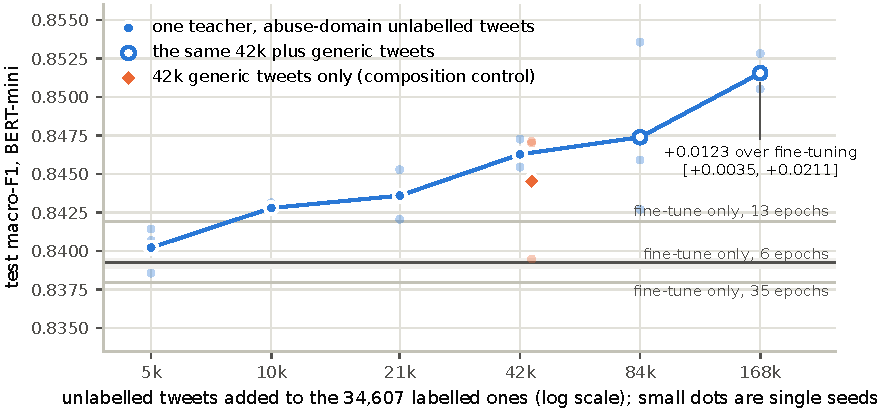
\includegraphics[width=\textwidth]{figures/fig_size_curve.pdf}
\caption[The size curve on BERT-mini]{The size curve on BERT-mini, one teacher labelling. Filled points: nested subsets of the abuse-domain transfer set; hollow points: the same set extended with generic tweets; diamond: 42,013 generic tweets alone. Horizontal lines: fine-tuning alone for 6, 13 and 35 epochs, the last two matching the number of updates of the 42k and 168k arms. Small dots are single seeds.}
\label{fig:size-curve}
\end{figure}

\textbf{The curve rises at every step} (Table~\ref{tab:size-curve}, Figure~\ref{fig:size-curve}).
Six sizes give six ordered means with no inversion, the 42k arm reproduces Section~\ref{sec:5.7}'s
to within 0.0003, and at 168k the gain is +0.0123 with an interval that excludes zero: the largest
gain in the grid on the headline student, and one of three arms that beat fine-tuning by more than
the test set can resolve. No single step of the curve is significant on its own (the largest, 84k to
168k, is +0.0042 [$-$0.0047, +0.0134]); the evidence is the ordering, and the endpoint.

\textbf{Composition matters less than we predicted.} We expected generic tweets of the same size to
gain at least 0.003 less than the abuse-domain set; they gain 0.0017 less (+0.0017 [$-$0.0066,
+0.0113]), with two of three seeds level with the abuse-domain arm. Text from the same platform
carries most of the value, which makes the recipe cheaper than we assumed: the unlabelled text need
not be abuse-related, only in the register the student will meet. Returns diminish, as predicted:
the abuse-domain rows added 1.7 points of macro-F1 per 10,000, the generic rows appended beyond them
0.4.

\textbf{Optimisation length does not explain the curve} (Figure~\ref{fig:validation}). Fine-tuning
for the 42k arm's number of updates gains +0.0027; fine-tuning for the 168k arm's number of updates
gains nothing, $-$0.0013 [$-$0.0106, +0.0072], with the validation score peaking between epochs 6
and 13 and declining afterwards (0.855 to 0.844 by the last epoch): the extra updates are spent
overfitting. The 13-epoch control's small gain was a longer search over checkpoints rather than a
better optimum, and 35 epochs is its ceiling. Against these controls the 42k arm keeps +0.0043
[$-$0.0032, +0.0122]; the 168k arm keeps +0.0096 [+0.0000, +0.0191] over the 13-epoch control and
+0.0136 [+0.0023, +0.0240], the latter with an interval clear of zero.

\begin{figure}[htbp]
\centering
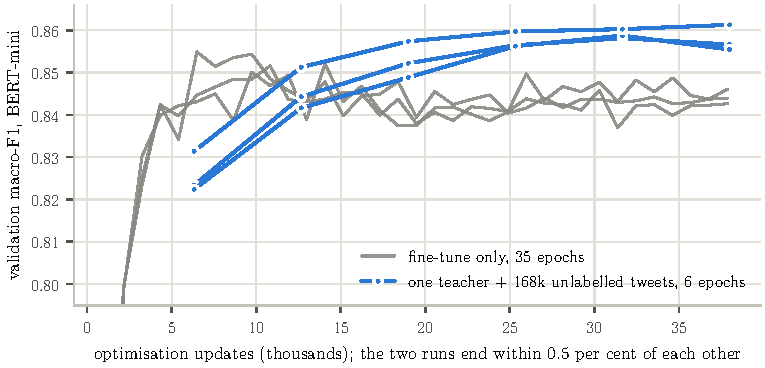
\includegraphics[width=\textwidth]{figures/fig_validation.pdf}
\caption[Validation macro-F1 against optimisation updates]{Validation macro-F1 of BERT-mini against the number of optimisation updates. Fine-tuning alone for 35 epochs (gray, three seeds) peaks early and then declines; the 168k transfer arm (blue, three seeds) reaches a higher score within the same number of updates.}
\label{fig:validation}
\end{figure}

\textbf{The endpoint holds on two more students} (Table~\ref{tab:students},
Figure~\ref{fig:students}). The largest set was run on BERT-small (28.8M, the same family) and on
the BiLSTM (10.4M, the heterogeneous student), beside their in-sample fine-tuning and single-teacher
runs:

\begin{table}[htbp]
\centering
\small
\caption{The largest transfer set on three students, three seeds each.}
\label{tab:students}
\begin{adjustbox}{max width=\textwidth}
\begin{tabular}{lccccc}
\toprule
Student & Fine-tune only & Single teacher, in sample & + 168k transfer rows & Gain over fine-tuning & Gain over the same teacher in sample \\
\midrule
BERT-mini (11.2M) & 0.8393 $\pm$ 0.0003 & 0.8405 $\pm$ 0.0017 & 0.8516 $\pm$ 0.0012 & +0.0123 [+0.0035, +0.0211] & +0.0111 \\
BERT-small (28.8M) & 0.8469 $\pm$ 0.0040 & 0.8488 $\pm$ 0.0044 & 0.8526 $\pm$ 0.0016 & +0.0057 [$-$0.0063, +0.0171] & +0.0038 [$-$0.0049, +0.0137] \\
BiLSTM (10.4M) & 0.8693 $\pm$ 0.0043 & 0.8748 $\pm$ 0.0018 & 0.8856 $\pm$ 0.0003 & +0.0163 [+0.0063, +0.0271] & +0.0108 [+0.0023, +0.0200] \\
\bottomrule
\end{tabular}
\end{adjustbox}
\end{table}

\begin{figure}[htbp]
\centering
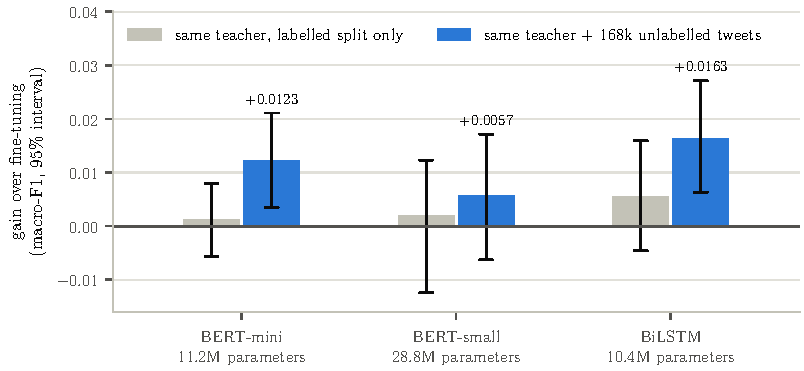
\includegraphics[width=\textwidth]{figures/fig_students.pdf}
\caption[The largest transfer set on three students]{Gain over fine-tuning from the same teacher, in sample and with 168,000 unlabelled tweets, on three students. Whiskers are paired bootstrap 95\% intervals.}
\label{fig:students}
\end{figure}

The BiLSTM gains most, every seed above every baseline seed, and at 10.4M parameters now clears the
classical floor (0.8798) and sits within 0.006 of DistilBERT's fine-tuning (0.8907) with a sixth of
the parameters. BERT-small gains on the mean, with two of three seeds above every fine-tuning seed,
but its fine-tuning seeds vary by 0.008 and its interval includes zero, which we report as it is. On
every student the gain lands in the same place: between fine-tuning and the 168k arm, F1 on
not\_cyberbullying rises from 0.644 to 0.671 on BERT-mini and from 0.690 to 0.734 on the BiLSTM, on
other\_cyberbullying from 0.707 to 0.720 and from 0.719 to 0.747, while the four targeted classes
move by at most 0.016. The unlabelled text teaches the boundary the labelled split draws worst.

The constructive sentence of this paper is therefore measured on four axes: the gain exists, it
grows with the unlabelled text, it comes from any tweets of the platform, and it holds on three
compact students of two families while fine-tuning for the same number of updates gains nothing.
What it does not have is a second corpus, which Chapter~\ref{ch:7} lists first.
\section{What Never Transferred: Discrimination of Implied Abuse Is Fixed by Pre-Training}
\label{sec:5.9}
\textbf{The failure is discrimination, not blindness.} Diagnostic on BERT-mini fine-tune-only, seed
1. Recall on the ironic-abuse probe is 0.91 on the 43 items containing explicit profanity and 0.76
on the 1,517 without; on the implicit-abuse probe 0.91 on 11 items with and 0.74 on 752 without.
Profanity helps, by 6 to 16 points of recall on every in-sample model analysed, but the items
without it are still caught about three times in four: the detector leans on profanity without being
a profanity detector. Mean $p(\text{abusive})$ is 0.748 on ironic abuse and 0.449 on benign sarcasm,
the distributions overlap heavily, and sarcasm-discrimination AUC is 0.773. At a 0.5 threshold,
recall of 0.792 costs a 39.5 per cent false-positive rate on sarcasm that attacks nobody. No
threshold up to 0.90 brings that rate under 10 per cent on any of the 29 in-sample models analysed;
three of the 14 out-of-sample and matched-steps models reach it at 0.90, at a recall of 0.31 to
0.39. The benchmark's own labels show the same confusion: other\_cyberbullying recall 0.710 with 109
of its errors going to not\_cyberbullying, and not\_cyberbullying recall 0.648 with 126 going the
other way.

\textbf{Nothing raises the discrimination} (Figure~\ref{fig:auc}). Over the 28 in-sample pre-trained
variants of BERT-mini analysed, which cover every objective and committee, seven temperatures, the
$T$, $\alpha$ and $\delta$ sweeps, every ablation and both controls, sarcasm-discrimination AUC has
mean 0.771 and standard deviation 0.004, from 0.756 to 0.777. The randomly initialised student
scores 0.613. The auxiliary irony head, the component built for this measurement, is inside the
band: without it 0.775, with it 0.773. Along the whole out-of-sample curve the first seed's AUC is
0.758, 0.764, 0.752, 0.765, 0.771 and 0.761, the generic control's 0.760, the 35-epoch control's
0.774 and the hard-label arm's 0.727: every pre-trained variant of the student lies between 0.72 and
0.78, and every soft-label variant between 0.75 and 0.78. This is where a pre-registered prediction
failed as written: the transfer run's predictions included the claim that the AUC would stay inside
the in-sample band of 0.756 to 0.777 on every arm, and three of the five arms fall below that band,
the hard-label arm furthest at 0.727. Nothing rises above it.

\begin{figure}[htbp]
\centering
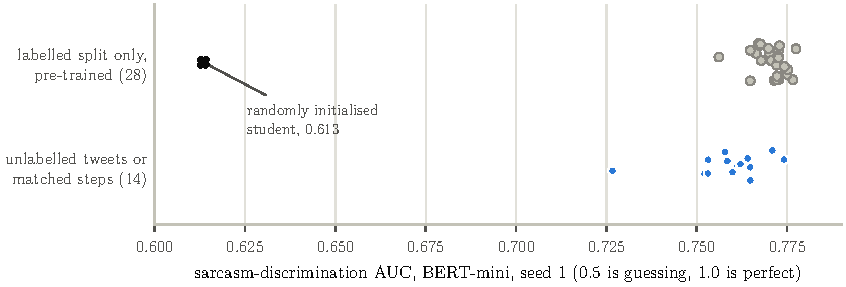
\includegraphics[width=\textwidth]{figures/fig_auc.pdf}
\caption[Sarcasm-discrimination AUC of every analysed variant]{Sarcasm-discrimination AUC of every analysed BERT-mini variant, first seed. Every pre-trained variant lies between 0.72 and 0.78, in sample or out; only removing pre-training moves the measure.}
\label{fig:auc}
\end{figure}

What moves is the operating point. Over the 28 pre-trained in-sample variants, recall at 0.5 ranges
from 0.758 to 0.821 and the false-positive rate from 0.343 to 0.448, correlated at +0.87; along the
out-of-sample curve both fall together, recall from 0.74 to 0.57 and the false-positive rate from
0.35 to 0.25 as the set grows to 168,000 rows, and on the BiLSTM to 0.50 and 0.18. The out-of-sample
student fires less on sarcasm of both kinds; it does not tell them apart any better.

\textbf{Across the grid, methods differ only in how readily they fire} (Figure~\ref{fig:tradeoff},
Table~\ref{tab:families}). Across all 184 evaluated models in the grid, teachers and students, every
mode and seed, the false-positive rate on benign sarcasm and the recall on ironic abuse correlate at
+0.772. Recall minus false-positive rate has mean 0.357 and standard deviation 0.046, while its
components range over 0.14 to 0.59 and 0.48 to 0.81. The 42 out-of-sample models do not leave the
curve, they slide along it: among themselves they correlate at +0.922, with the same mean margin,
0.355.

\begin{figure}[htbp]
\centering
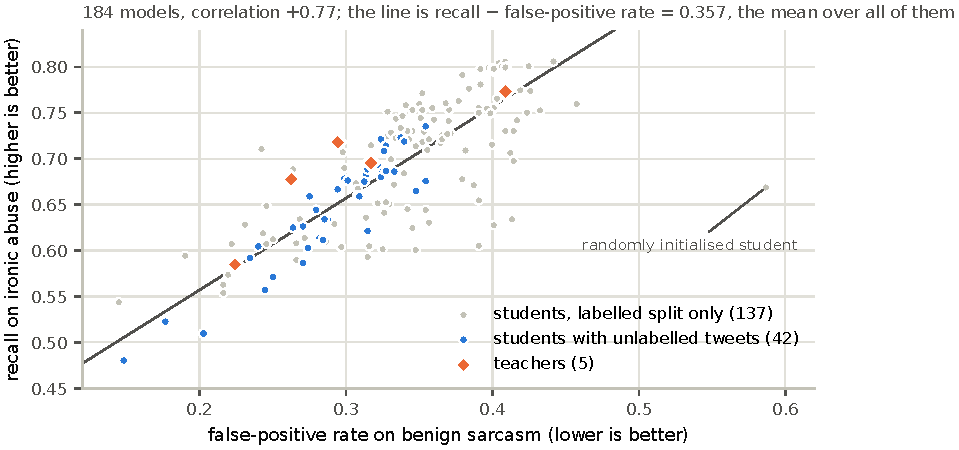
\includegraphics[width=\textwidth]{figures/fig_tradeoff.pdf}
\caption[False-positive rate against recall, all 184 models]{False-positive rate on benign sarcasm against recall on ironic abuse for all 184 evaluated models. Every family and objective lies along one trade-off line; the out-of-sample students slide along it rather than rising above it.}
\label{fig:tradeoff}
\end{figure}

\begin{table}[htbp]
\centering
\small
\caption[Probe metrics by model family]{Probe metrics by model family, averaged over all 184 evaluated models, at each model's argmax decision. The margin is recall minus false-positive rate.}
\label{tab:families}
\begin{adjustbox}{max width=\textwidth}
\begin{tabular}{lcccc}
\toprule
Model family & n & Benign FPR & Ironic recall & Margin \\
\midrule
DeBERTa-v3-xsmall & 21 & 0.334 & 0.728 & 0.394 \\
Teachers & 5 & 0.301 & 0.690 & 0.388 \\
DistilBERT & 21 & 0.238 & 0.607 & 0.369 \\
BERT-mini & 89 & 0.350 & 0.718 & 0.368 \\
BERT-small & 24 & 0.369 & 0.700 & 0.332 \\
BiLSTM & 24 & 0.316 & 0.608 & 0.292 \\
\bottomrule
\end{tabular}
\end{adjustbox}
\end{table}

Distillation mode does not appear in this ordering; architecture does. The models occupy different
points on one trade-off curve rather than different curves, and the worst margin in the grid, 0.082,
belongs to the randomly initialised student. Whatever ability these models have to tell implied
abuse from harmless sarcasm comes from pre-training, and nothing added to the objective or to the
data moves it. This is why the paper reports a threshold-free area: recall at a fixed cut measures
how readily a model fires, and across 184 models that is all it measures.

\textbf{The same failure on a corpus that labels implication} (Table~\ref{tab:implicit}).

\begin{table}[htbp]
\centering
\small
\caption{The implicit benchmark: the compact student, the specialist and the classical floor, one seed.}
\label{tab:implicit}
\begin{adjustbox}{max width=\textwidth}
\begin{tabular}{lccccc}
\toprule
Model & macro-F1 & not\_hate F1 & explicit\_hate F1 & implicit\_hate F1 & Implicit-discrimination AUC \\
\midrule
Classical floor & 0.5620 & -- & -- & 0.5562 & 0.7610 \\
BERT-mini, fine-tune only & 0.5549 & 0.8347 & 0.2857 & 0.5443 & 0.8196 \\
HateBERT specialist & 0.6029 & 0.8352 & 0.3662 & 0.6072 & 0.8247 \\
\bottomrule
\end{tabular}
\end{adjustbox}
\end{table}

The compact student loses to a bag of n-grams on F1 and beats it decisively on ranking: it separates
implied abuse from benign text at 0.8196 AUC against 0.7610 while scoring below the floor on the
implicit class itself. The two measures disagree in direction, not degree, which is the argument of
this section made on other people's labels. Both neural models score 0.29 to 0.37 on the 108-row
explicit class, which is why macro-F1 is not the headline here; these are single-seed results.
Applied without further training to the benchmark's 2,064 test posts, the tweet-trained BERT-mini
calls 81.0 per cent of them abusive against a true rate of 35.7 per cent (binary macro-F1 0.423,
ROC-AUC 0.608). On implicit hate against posts that are not hateful it catches 85.1 per cent at a
78.8 per cent false-positive rate. It ranks the two at an AUC of 0.600, barely above chance, against
0.820 for the same architecture trained on the corpus. D-MTHD transfers no better: binary macro-F1
0.411, the same two AUCs at 0.609 and 0.600. Whatever the tweet students have learned about abuse,
in sample or out, does not include what makes an implication hateful; there was little of that
knowledge in the committee to receive, and none in the transfer text.
\section{Character-Level Obfuscation and Deployment Cost}
\label{sec:5.10}
Table~\ref{tab:robustness} gives macro-F1 under synthetic obfuscation of the abusive test rows, on
BERT-mini, seed 1.

\begin{table}[htbp]
\centering
\small
\caption[Macro-F1 under character-level obfuscation]{Macro-F1 under synthetic character-level obfuscation of the abusive test rows: letters replaced by digits, adjacent characters swapped, spaces inserted, and all three together. BERT-mini, seed 1.}
\label{tab:robustness}
\begin{adjustbox}{max width=\textwidth}
\begin{tabular}{lccccc}
\toprule
Objective & Clean & Leetspeak & Character swap & Inserted spaces & Mixed \\
\midrule
Fine-tune only & 0.8394 & 0.7475 & 0.7417 & 0.7275 & 0.7116 \\
D-MTHD & 0.8385 & 0.7460 & 0.7361 & 0.7250 & 0.7077 \\
\bottomrule
\end{tabular}
\end{adjustbox}
\end{table}

Nine to thirteen points lost on short text, and distillation does not help: the two objectives are
within 0.006 of each other under every edit. These are character edits, not evasion by people trying
to evade, and we do not call the result robustness.

Table~\ref{tab:efficiency} gives the median of five timed passes after warm-up on an idle machine.

\begin{table}[htbp]
\centering
\small
\caption[Deployment profile of the students and the largest teacher]{Deployment profile of the students and the largest teacher: parameters, latency at batch sizes 1 and 32, FLOPs per sequence, model size, and macro-F1 after INT8 dynamic quantisation.}
\label{tab:efficiency}
\begin{adjustbox}{max width=\textwidth}
\begin{tabular}{lccccccc}
\toprule
Student & Params & Latency b1 & Latency b32 & GFLOPs/seq & fp32 size & INT8 size & INT8 macro-F1 \\
\midrule
BiLSTM & 10.4M & 2.57 ms & 0.18 ms & $\sim$0 & 40 MB & 32 MB & 0.8736 \\
BERT-mini & 11.2M & 3.47 ms & 0.37 ms & 0.87 & 43 MB & 33 MB & 0.8319 \\
BERT-small & 28.8M & 3.74 ms & 1.25 ms & 3.36 & 110 MB & 73 MB & 0.8448 \\
DistilBERT & 67.0M & 5.22 ms & 3.72 ms & 11.17 & 255 MB & 132 MB & 0.8931 \\
DeBERTa-v3-xsmall & 70.8M & 23.49 ms & 3.25 ms & 10.57 & 270 MB & 209 MB & 0.8765 \\
BERT-large (teacher) & 335.1M & 26.56 ms & 21.65 ms & 78.92 & 1,279 MB & -- & -- \\
\bottomrule
\end{tabular}
\end{adjustbox}
\end{table}

DistilBERT matches BERT-large at 5.0 times fewer parameters and 5.8 times lower batch-32 latency;
INT8 dynamic quantisation halves its size for 0.003 macro-F1. BERT-mini's size falls only from 43 to
33 MB because 7.8M of its 11.2M parameters are the embedding table, which dynamic quantisation does
not touch. The out-of-sample recipe adds nothing to inference: the transfer set is used once, in
training, and the deployed student is the same model.

\section{The Research Questions, Decided}
\label{sec:5.11}
The four questions of Section~\ref{sec:1.4} are decided here on the measurements above, under one rule
fixed before any of them was run: a difference counts only if its paired bootstrap interval excludes
zero, and on a test set of 4,326 posts that requires roughly 0.007 macro-F1 (Section~\ref{sec:4.7}).
Table~\ref{tab:rq} states each decision beside the evidence that carries it; the paragraphs below give
the numbers. Chapter~\ref{ch:6} takes up what the decisions mean.

\begin{table}[htbp]
\centering
\footnotesize
\caption[The four research questions and their decisions]{Each research question, the rule that decides
it, the measurement that decides it, and the decision.}
\label{tab:rq}
\begin{adjustbox}{max width=\textwidth}
\begin{tabular}{p{2.0cm}p{3.5cm}p{5.6cm}p{2.3cm}}
\toprule
Question & Decided by & Measurement & Decision \\
\midrule
RQ1: does the weighted committee beat no teacher at all, in sample? & Any interval excluding zero among
the in-sample distillation-against-fine-tuning comparisons & 27 such comparisons, none excludes zero;
best of six per student is $+0.0012$ to $+0.0071$, five intervals of five containing zero; weighting
minus averaging is $-0.0034$ to $+0.0000$, every interval containing zero & \textbf{No}
(Sections~\ref{sec:5.2}, \ref{sec:5.3}, \ref{sec:5.5}) \\
RQ2: what explains that? & The mechanism has to be measured, not argued & Teachers end training at loss
0.033 to 0.077 on the split the student is distilled on; weights 0.332 / 0.337 / 0.331 against a uniform
0.333, and 0.318 / 0.356 / 0.326 even at $\tau = 0.05$; pairwise $\kappa$ 0.889 to 0.962, all four
teachers right on 83.2 per cent of the test set and wrong together on 4.7 & \textbf{Memorised labels,
saturated weights, spent diversity} (Sections~\ref{sec:5.4}, \ref{sec:5.6}) \\
RQ3: does unlabelled text the teachers never saw help, and how? & Decision D20, written before the run:
the 168k arm gains at least 0.012 with the interval clear of zero and still rising & $+0.0123$ [$+0.0035$,
$+0.0211$] at 168,000 tweets, monotone over six sizes from $+0.0010$ at 5,000; generic text within
$+0.0017$ [$-0.0066$, $+0.0113$] of abuse-domain text at the same size; fine-tuning for the same updates
$-0.0013$ [$-0.0106$, $+0.0072$]; BiLSTM $+0.0163$ [$+0.0063$, $+0.0271$] & \textbf{Yes, and it is the
text} (Sections~\ref{sec:5.7}, \ref{sec:5.8}) \\
RQ4: does any of it improve the reading of implication? & A threshold-free AUC rising above the
in-sample band of 0.756 to 0.777 & 28 in-sample pre-trained variants, mean 0.771, standard deviation
0.004; out-of-sample arms 0.727 to 0.771, three below the band and none above; the randomly initialised
student 0.613; across 184 models recall and false-positive rate correlate at $+0.772$ & \textbf{No}
(Section~\ref{sec:5.9}) \\
\bottomrule
\end{tabular}
\end{adjustbox}
\end{table}

\textbf{RQ1 is decided against the method.} The grid makes 27 in-sample comparisons of a distilled
student against the same student fine-tuned without teachers, and no interval excludes zero. Taking the
best of six configurations per student, which flatters the method, gives $+0.0012$, $+0.0040$,
$+0.0068$, $+0.0040$ and $+0.0071$ macro-F1, all five intervals containing zero and all five below the
0.007 the test set can resolve. Per-instance weighting against uniform averaging gives $-0.0007$,
$-0.0034$, $+0.0000$, $-0.0029$ and $-0.0029$, and across a hundredfold range of $\tau$ the headline
student moves by 0.0007 and stays under fine-tuning at every value. Adding a teacher trained on labelled
implication changes it by $+0.0005$ [$-0.0059$, $+0.0064$] under averaging and $-0.0005$ [$-0.0069$,
$+0.0055$] under weighting. The answer is no at this resolution, and Section~\ref{sec:7.1} records that
an absence at this resolution is not a zero.

\textbf{RQ2 is decided by three measurements rather than by argument.} Four of the five teachers end
their last epoch at a cross-entropy between 0.033 and 0.077 on the split the weights are read from and
the student is distilled on, so their soft labels carry what the gold labels already carry; the one
teacher that did not memorise the split, DeBERTa at 0.227, is the one whose weight moves, to 0.233 in a
committee of four. The weights are therefore flat at every temperature the sweep reaches. And the
committee has little to route between: pairwise agreement runs from $\kappa = 0.889$ to $0.962$, the
four original teachers are right together on 83.2 per cent of the test set and wrong together on 4.7,
and no combination rule that sees only their probabilities, including a stacked gate fitted by
cross-validation on the test set, improves on their uniform mean by more than 0.005 against an oracle
sitting 4 to 5 accuracy points higher.

\textbf{RQ3 is decided for the data and against the committee.} Decision D20 fixed the rule before the
run: if the largest arm gained at least 0.012 with an interval clear of zero and the curve was still
rising, the constructive result would lead. It gained $+0.0123$ [$+0.0035$, $+0.0211$], the six sizes
are ordered without inversion from $+0.0010$ at 5,000 tweets, and the curve had not flattened. The three
controls hold: generic tweets of the same size come within $+0.0017$ [$-0.0066$, $+0.0113$] of
abuse-domain ones, fine-tuning for the same number of updates gains $-0.0013$ [$-0.0106$, $+0.0072$],
and the gain reappears on a second and third student, $+0.0163$ [$+0.0063$, $+0.0271$] on the BiLSTM and
$+0.0057$ [$-0.0063$, $+0.0171$] on BERT-small. The committee is not part of it: against a single
teacher on the same text it is $-0.0003$ [$-0.0061$, $+0.0056$], its corrected weighting adds $+0.0021$
[$-0.0017$, $+0.0082$], and its hard pseudo-labels gain $+0.0020$ against $+0.0070$ for its soft ones.

\textbf{RQ4 is decided against every intervention in the grid.} Measured without a threshold, 28
in-sample pre-trained variants of the headline student, covering every objective, committee,
temperature, sweep, ablation and control, have a sarcasm-discrimination AUC of mean 0.771 and standard
deviation 0.004. The out-of-sample arms run from 0.727 to 0.771: three of five fall below that band and
none rises above it, which is also where a pre-registered prediction failed as written. The only
intervention that moves the measure is removing pre-training, which drops it to 0.613. Across all 184
evaluated models recall on ironic abuse and the false-positive rate on benign sarcasm correlate at
$+0.772$ with a margin of $0.357 \pm 0.046$, so what the interventions change is where a model sits on
one trade-off line, not which line it is on. On a corpus that labels implication the same students rank
implied abuse against benign text at 0.600 to 0.609 AUC, against 0.820 for the same architecture trained
on that corpus.
